\documentclass[11pt]{article}
\usepackage{../EllioStyle}
\usepackage{listings}

\definecolor{codegreen}{rgb}{0,0.6,0}
\definecolor{codegray}{rgb}{0.5,0.5,0.5}
\definecolor{codepurple}{rgb}{0.58,0,0.82}
\definecolor{backcolour}{rgb}{0.95,0.95,0.92}

\graphicspath{ {imgs/} }

\title{Homework 2}
\author{Elliott Pryor}
\date{30 October 2023}

\rhead{Homework 2}

\begin{document}
\maketitle

My work can be found on my github:
\href{https://github.com/ElliottP-13/DeepRL-Course/tree/main/hw1}{https://github.com/ElliottP-13/DeepRL-Course}.

There is not any explicit question given, besides to run
\begin{lstlisting}[language=Bash]
$ python ds6559/scripts/run_hw2.py --env_name CartPole-v0 --exp_name test_cartpole \
    --video_log_freq -1
$ python ds6559/scripts/run_hw2.py --env_name InvertedPendulum-v4 \
    --exp_name test_pendulum --video_log_freq -1
\end{lstlisting}

So my results from the first command can be seen in Figure \ref{fig:one} and the second command can be seen in Figure \ref{fig:two}.
\begin{figure}[h] 
    \centering
    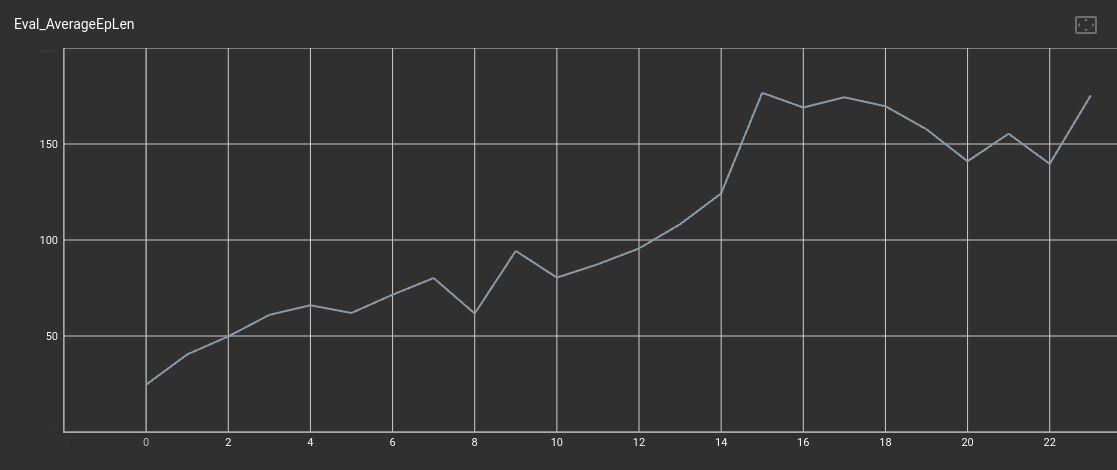
\includegraphics[width=0.75 \linewidth]{10-30-1_eplen}
    \caption{Command 1}
    \label{fig:one}
\end{figure}

\begin{figure}[h] 
    \centering
    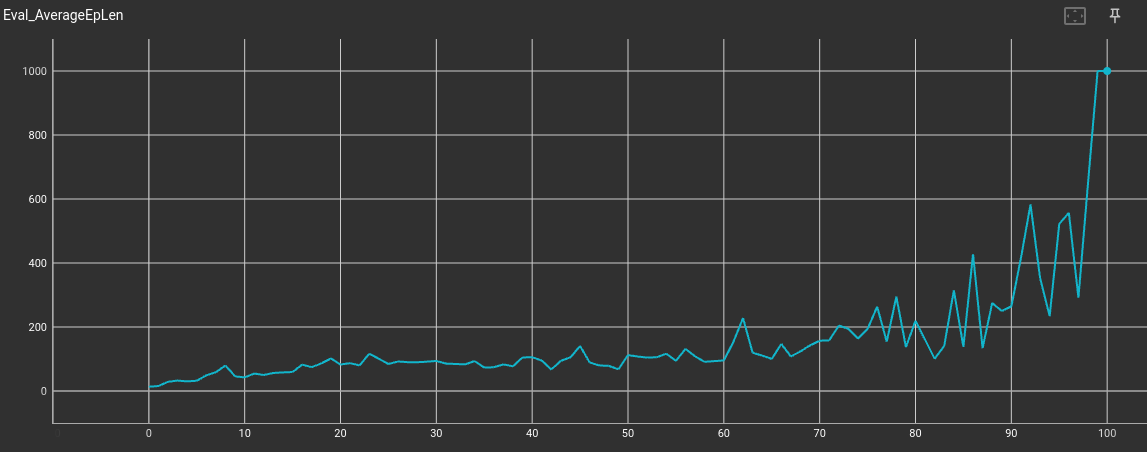
\includegraphics[width=0.75 \linewidth]{10-30-2_eplen}
    \caption{Command 2}
    \label{fig:two}
\end{figure}

Because of the normalization that was asked to do in the code,
the program terminates once the optimal policy is reached.
This is because max number of environment steps are achieved in all the rollouts,
so the standard deviation is zero, thus normalization breaks.

For the first environment, there are only 200 timesteps, and 
and optimal policy is learned in 24 iterations. 
The second environment has max timesteps of 1000 which is learned in 103 iterations.

A video of the last cartpole rollout can be found at:

\href{https://github.com/ElliottP-13/DeepRL-Course/blob/main/Writeup/imgs/cartpole.mp4}{https://github.com/ElliottP-13/DeepRL-Course/blob/main/Writeup/imgs/cartpole.mp4}

\end{document}